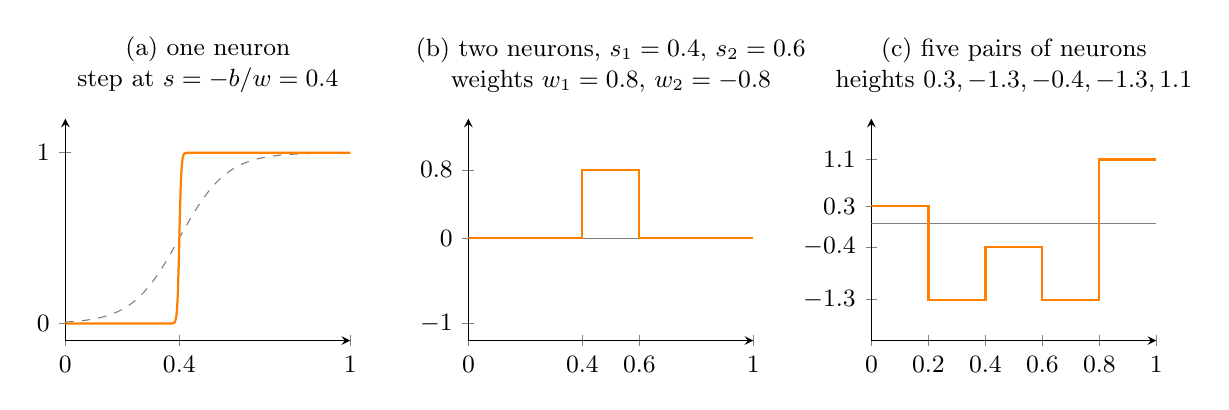
\begin{tikzpicture}[font=\small]
  \begin{axis}[name=A, width=5.2cm, height=4.4cm, xmin=0, xmax=1, ymin=-0.1, ymax=1.2,
      axis lines=left, xtick={0,0.4,1}, ytick={0,1},
      title={(a) one neuron\\ step at $s=-b/w=0.4$}, title style={font=\small, align=center}]
    \addplot[gray, dashed, domain=0:1, samples=120] {1/(1+exp(-12*(x-0.4)))};
    \addplot[orange, thick, domain=0:1, samples=300] {1/(1+exp(-300*(x-0.4)))};
  \end{axis}
  \begin{axis}[name=B, at={(A.east)}, anchor=west, xshift=1.5cm,
      width=5.2cm, height=4.4cm, xmin=0, xmax=1, ymin=-1.2, ymax=1.4,
      axis lines=left, xtick={0,0.4,0.6,1}, ytick={-1,0,0.8},
      title={(b) two neurons, $s_1=0.4$, $s_2=0.6$\\ weights $w_1=0.8$, $w_2=-0.8$}, title style={font=\small, align=center}]
    \addplot[gray, thin, domain=0:1] {0};
    \addplot[orange, thick, const plot] coordinates {(0,0) (0.4,0.8) (0.6,0) (1,0)};
  \end{axis}
  \begin{axis}[name=C, at={(B.east)}, anchor=west, xshift=1.5cm,
      width=5.2cm, height=4.4cm, xmin=0, xmax=1, ymin=-2, ymax=1.8,
      axis lines=left, xtick={0,0.2,0.4,0.6,0.8,1}, ytick={-1.3,-0.4,0.3,1.1},
      title={(c) five pairs of neurons\\ heights $0.3,-1.3,-0.4,-1.3,1.1$}, title style={font=\small, align=center}]
    \addplot[gray, thin, domain=0:1] {0};
    \addplot[orange, thick, const plot] coordinates {(0,0.3) (0.2,-1.3) (0.4,-0.4) (0.6,-1.3) (0.8,1.1) (1,1.1)};
  \end{axis}
\end{tikzpicture}
